%\newpage

\subsection{Making Racket More Portable With Linklets}
\label{subsec:racket}

\begin{figure}[h!]
  \centering
  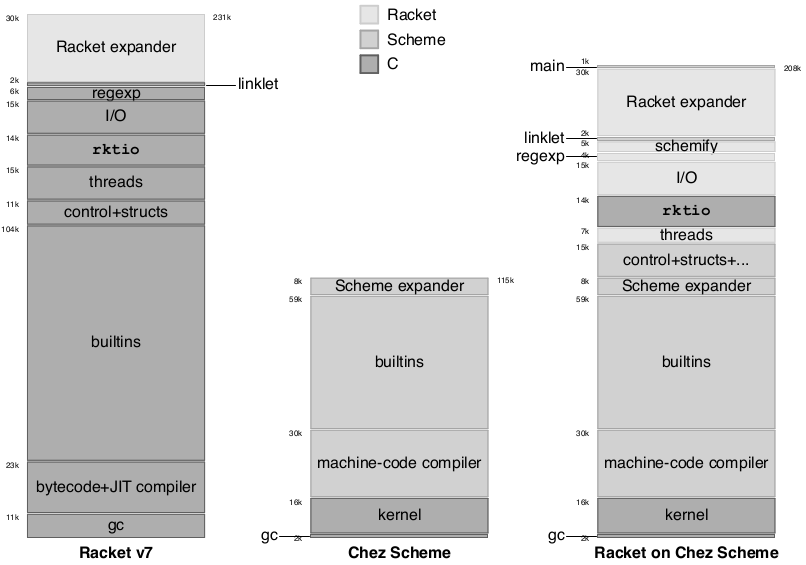
\includegraphics[scale=0.3]{img/racket-portable}
  \caption{Comparison of Racket implementations. Figure used
  from \cite{racket-on-chez-19}}
  \label{fig:racket-portable}
\end{figure}

In this section, we study how Racket became more portable to easily
re-target different virtual machines. I will present the general idea
and introduce the use of linklets as an essential part of a
communication language between the language and the run-time. Then I
will provide and example that demonstrates how functionalities such as
the top-level are implemented in this setup. Next I will provide the
formalism for linklets that allows us to easily reason about and
implement them on VMs.

\inputsec{racket-expand}
\vspace{-0.25cm}
\inputsec{toplevel-example}

%\inputsec{on-portability}

\inputsec{linklets-semantics}
